\documentclass{ltjsarticle} %lualatex cs_jikken.texで作成 
\usepackage{mdframed}
\usepackage{graphicx}
\usepackage{float}
\usepackage{array}
\usepackage{tikz}
\usepackage{circuitikz}
\usetikzlibrary{automata, positioning, arrows}
\begin{document}

\thispagestyle{empty}
\begin{flushright}
{\large 実験実施日 2024年10月31日{\hspace{5cm}}} 
\end{flushright}

\vspace*{\fill}
\centering
{\Huge\bf コンピュータ科学実験b}
\vspace*{1cm}

{\huge\bf ソフトウェア実験 第3,4週レポート}
\vspace*{\fill}

\vspace*{\fill}

\vspace*{\fill}

\begin{flushright}
{\large 学生番号: 102210017} \\ % 5cmの空白を作り、アンダーラインを引く
{\large 氏名: 安藤 駿} \\

{\large 共同実験者: 太田 充洋, 草島 悠伸, 阪口 修吾} \\
\end{flushright}

\clearpage

\addtocounter{page}{-1}
\raggedright
\setlength{\parindent}{1em}

\section{はじめに}
情報通信ネットワークは,現代の様々な計算機利用において必要不可欠のものとなっている.
本実験では, Python WSGI を用いて, SQL データベースと連携したWEBアプリケーションを作成し, ネットワークプ
ログラミングの基礎を学習する. 


\section{課題6 WEBアプリケーションの作成}

\subsection{目的・概要}
WEBサーバ上でSQLデータベースと協調して動作するWEBアプリケーションをPython言語で作成する. 

\subsection{作成したアプリケーションの概要と機能の説明}
作成したアプリケーションの概要と機能の説明をする. 

\subsubsection{アプリケーションの概要}
今回作成したアプリケーションは, WSGI(Web Server Gateway Interface)を使用し, sqlite3を用いて, 
気象庁の公式サイトから入手した愛知県名古屋市の天気と気温をデータベースで管理している. 
(気象庁, 2024)

\subsubsection{アプリケーションの機能}
このアプリケーションは, 日付, 気温, 天気の値を持つテーブルを作り, 気象庁の公式サイトから入手したcsvファイル
からレコードを作成することで, データベースを管理している. 

このアプリケーションには, データの検索, 登録, 削除の機能がある. 
データの検索は, 条件に適するレコードのみを表示する機能である. 
登録は, 入力した各フィールドの値を持つレコードを作成する機能である. 
削除は, 条件に適するレコードをテーブルから削除する機能である. 


\subsection{サービスの利用方法}
作成したアプリケーションの利用方法を説明する. 

\subsubsection{起動方法}
まず, 同じディレクトリ内に「102210017.wsgi」とディレクトリ「data」,「static」を入れる. 
ディレクトリ「data」内には, 入手した「data.csv」を入れる. 
ディレクトリ「static」内には, 「default.css」を入れる. 

ICE端末にSSH接続をし, 「python3 102210017.wsgi」を実行する. 
その後firefoxで, 「http://localhost:50017」にアクセスすると, 図\ref{fig:1}のようなウェブページが表示される. 

\begin{figure}[H] % 画像を挿入する環境を開始
  \centering
  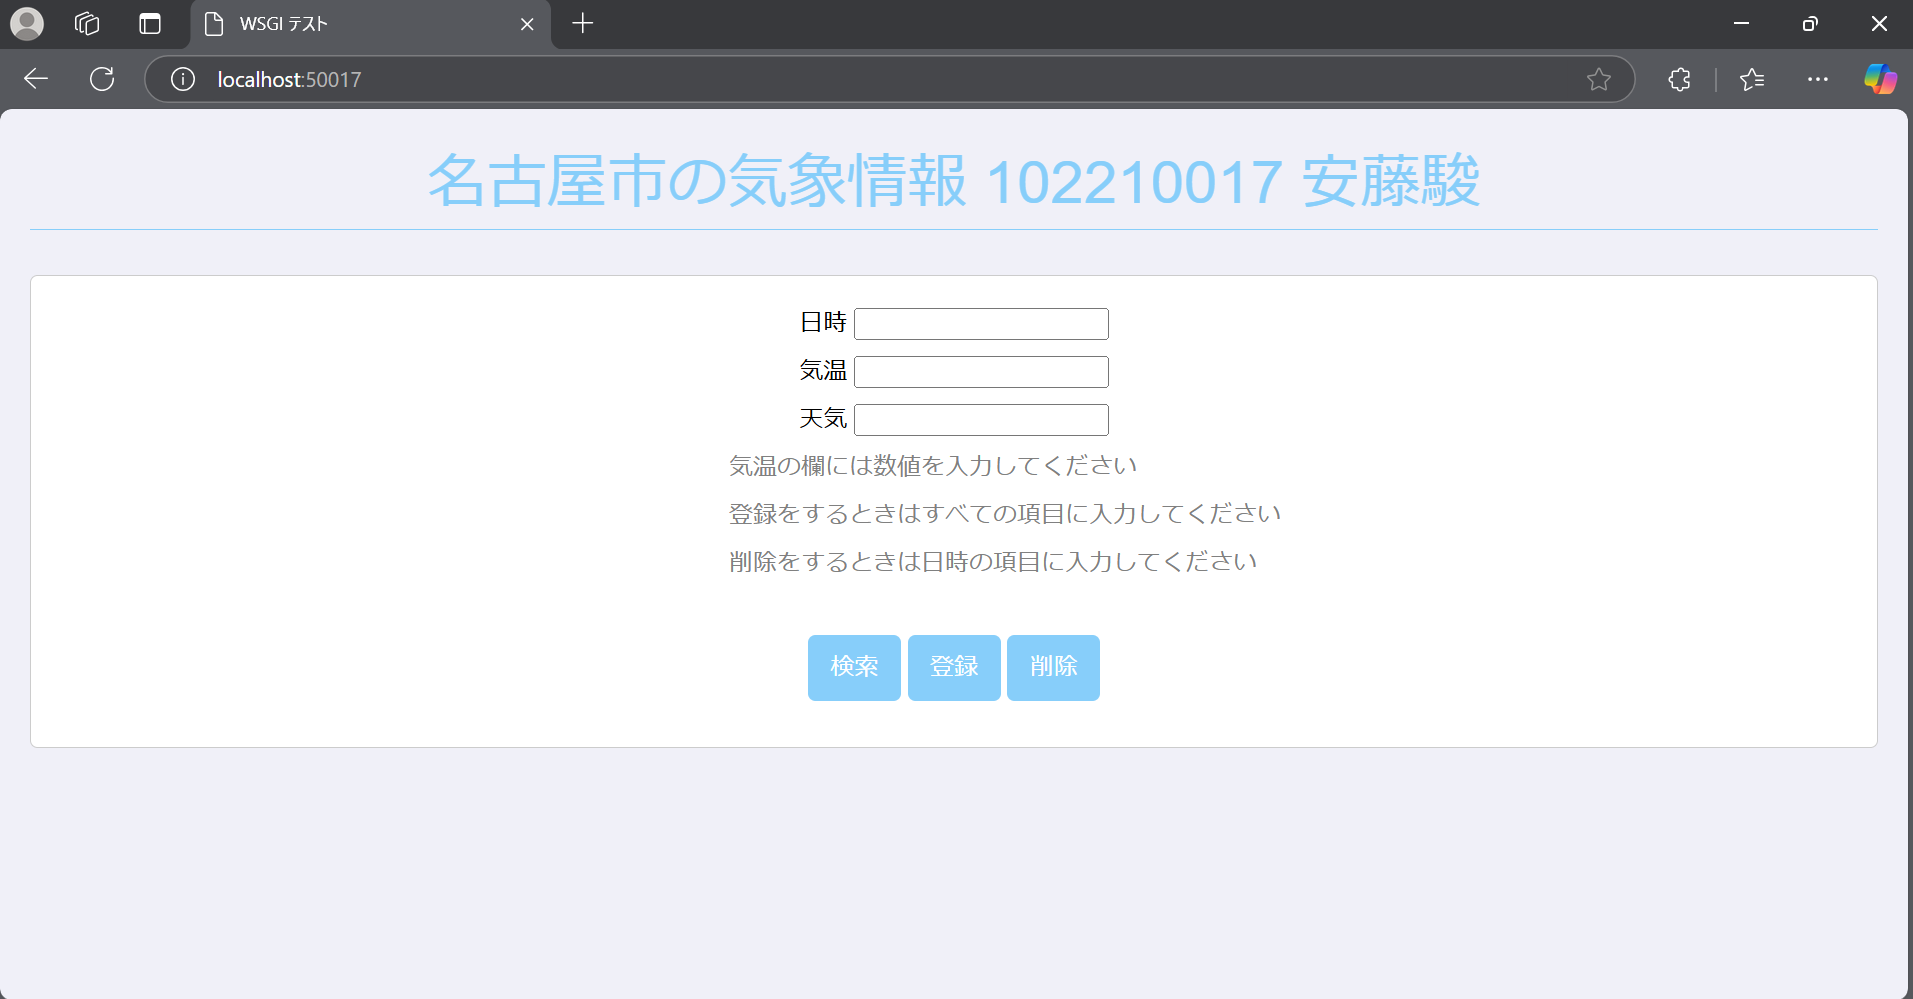
\includegraphics[width=1.0\textwidth]{1.png} % 画像を挿入、幅をページ幅に合わせる
  \caption{localhost:50017にアクセスした様子} % キャプションを追加
  \label{fig:1} % ラベルを追加
\end{figure}

\subsubsection{操作方法1 検索}
検索の機能について説明する. 入力欄に「晴」と入力し検索ボタンを押すと, 天気が「晴」のレコードの見つかった件数とその一覧が表示される. 
この時の状況を図\ref{fig:2}, \ref{fig:3}に示す. また, 日付や気温を入力しても同様に検索できる. 

気温の欄にfloat型に変換できない文字列を入力すると警告文が表示される. 気温の欄に「あああ」と入力し, 検索ボタンを押したときの
状況を図\ref{fig:4}に示す. 

\begin{figure}[H] % 画像を挿入する環境を開始
  \centering
  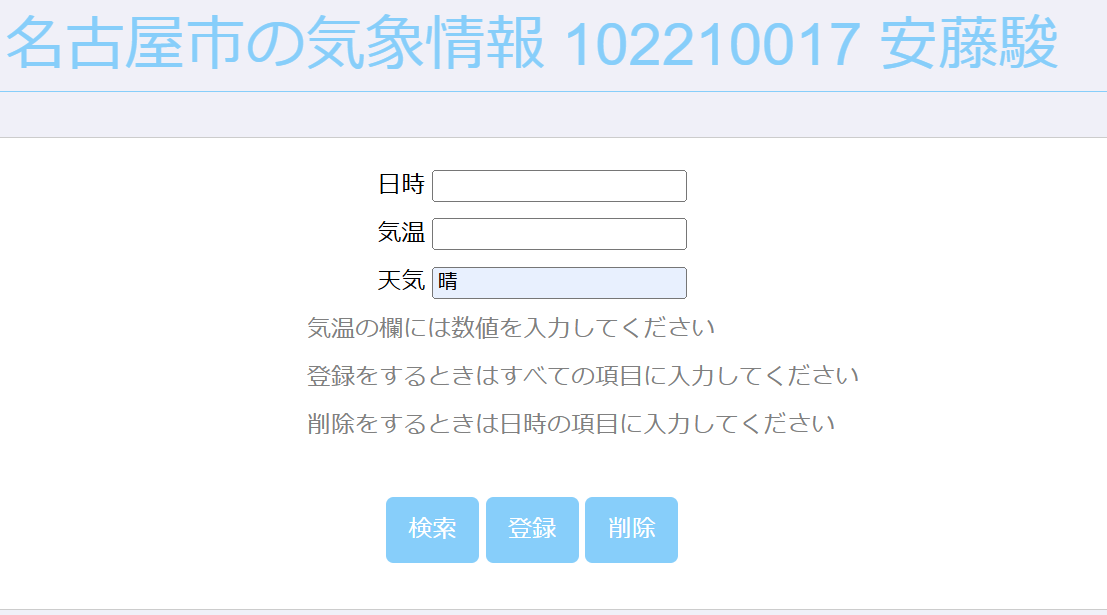
\includegraphics[width=0.8\textwidth]{2.png} % 画像を挿入、幅をページ幅に合わせる
  \caption{検索条件の入力} % キャプションを追加
  \label{fig:2} % ラベルを追加
\end{figure}

\begin{figure}[H] % 画像を挿入する環境を開始
  \centering
  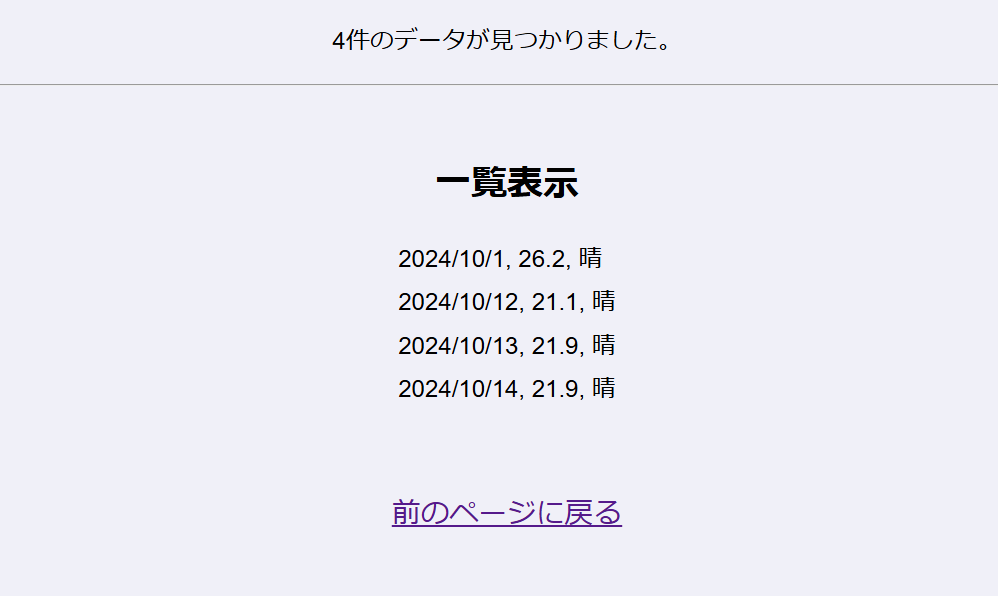
\includegraphics[width=0.8\textwidth]{3.png} % 画像を挿入、幅をページ幅に合わせる
  \caption{検索結果} % キャプションを追加
  \label{fig:3} % ラベルを追加
\end{figure}

\begin{figure}[H] % 画像を挿入する環境を開始
  \centering
  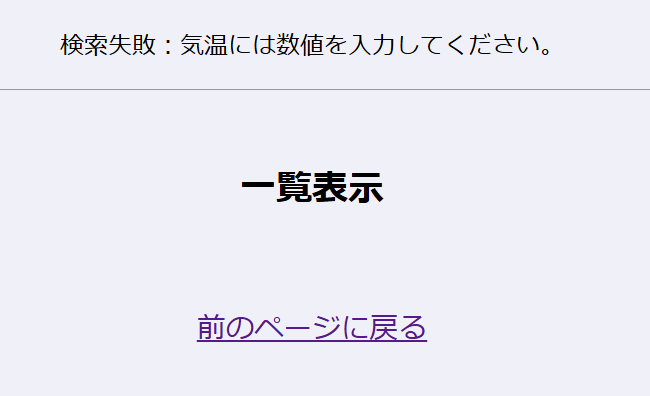
\includegraphics[width=0.8\textwidth]{4.png} % 画像を挿入、幅をページ幅に合わせる
  \caption{気温の入力に対する警告} % キャプションを追加
  \label{fig:4} % ラベルを追加
\end{figure}

\subsubsection{操作方法2 登録}
登録の機能について説明する. 入力欄に「2024/12/5」,「23.5」,「晴」と入力し登録ボタンを押すと, レコードの一覧が表示され, 
その最後尾に新しく作成したレコードが追加される. この時の状況を図\ref{fig:5}, \ref{fig:6}に示す. 

日付, 気温, 天気の入力欄のどれか一つに値を入れていないと, 警告文が表示される. 
また, 検索のときと同様に気温の欄にfloat型に変換できない文字列を入力すると, 警告文が表示される. 


\begin{figure}[H] % 画像を挿入する環境を開始
  \centering
  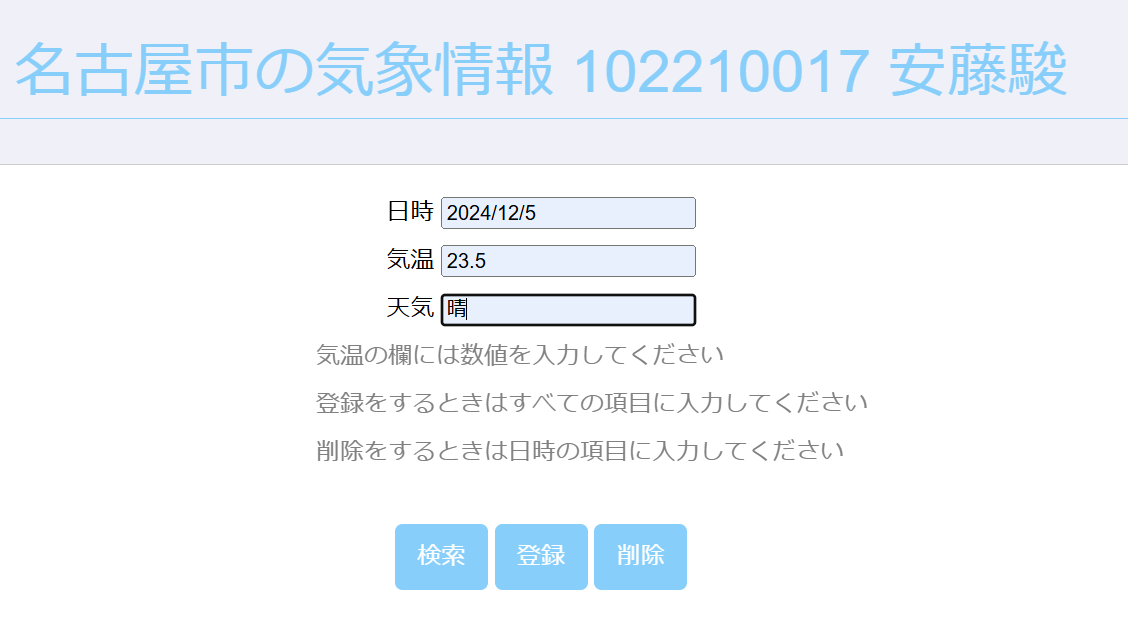
\includegraphics[width=0.8\textwidth]{5.png} % 画像を挿入、幅をページ幅に合わせる
  \caption{登録条件の入力} % キャプションを追加
  \label{fig:5} % ラベルを追加
\end{figure}

\begin{figure}[H] % 画像を挿入する環境を開始
  \centering
  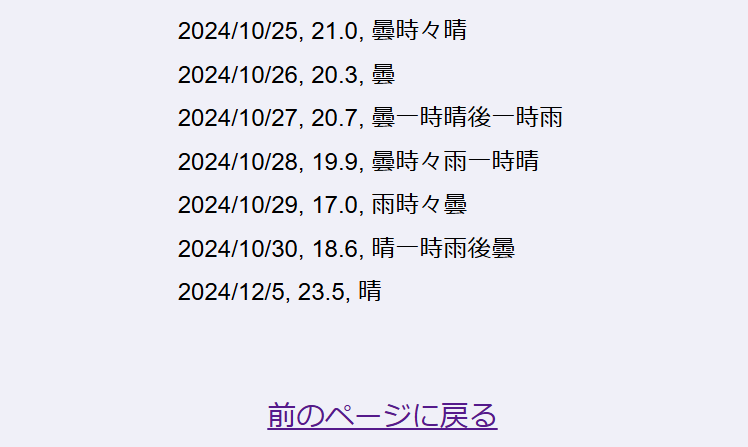
\includegraphics[width=0.8\textwidth]{6.png} % 画像を挿入、幅をページ幅に合わせる
  \caption{登録結果} % キャプションを追加
  \label{fig:6} % ラベルを追加
\end{figure}

\subsubsection{操作方法3 削除}
削除の機能について説明する. 日付の欄にのみ値を入力し, 削除ボタンを押すとその日付のレコードがすべて削除される. 
検索や登録とは違い, 気温, 天気による削除はできない. 

気温の欄に「2024/10/5」と入力し, 削除ボタンを押した時の状況を図\ref{fig:7}に示す. 

\begin{figure}[H] % 画像を挿入する環境を開始
  \centering
  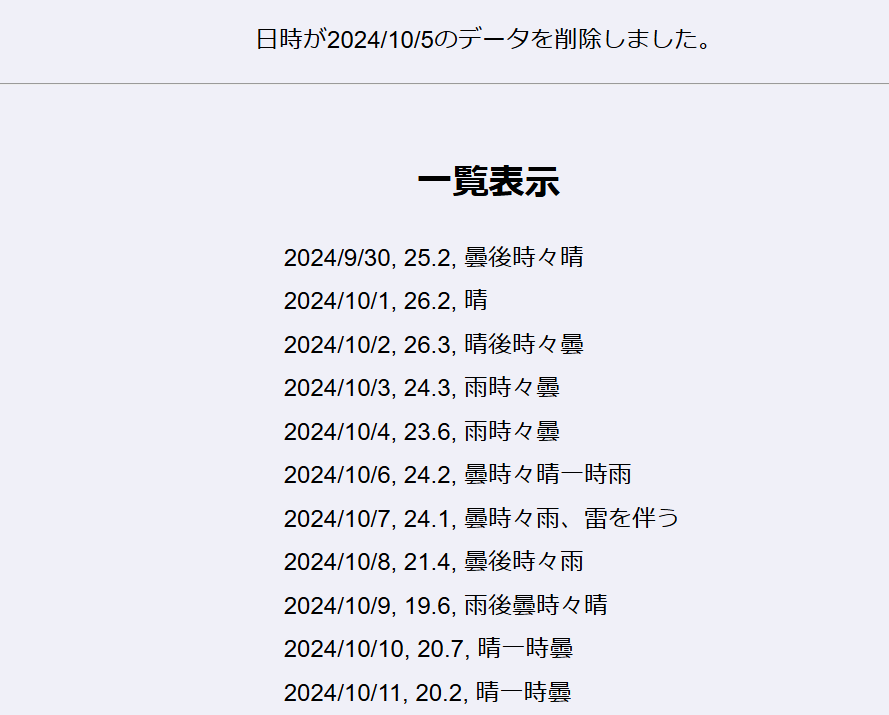
\includegraphics[width=0.8\textwidth]{7.png} % 画像を挿入、幅をページ幅に合わせる
  \caption{削除結果} % キャプションを追加
  \label{fig:7} % ラベルを追加
\end{figure}

\subsection{工夫した点}
気温の欄にfloatに変換できない値を入力したときにエラーになってしまったので, これに対応するために
「try except」を用いて, 警告文を表示できるようにした. 

\subsection{未解決のバグ}
二回目以降に「python3 102210017.wsgi 50017」を実行したときにデータベースに再びcsvファイルから
データが読み込まれ, レコードが作成されてしまうことがあった. 毎回このバグが起こるわけではく, 発生する条件がよくわからなかった. 

\section{調査課題6}
Webアプリケーションのセキュリティを脅かす代表的な脆弱性について調査した. 

\subsection{SQLインジェクション}
SQLインジェクションとは, 入力フォームやURLパラメータなどから入力した「SQL文を含む文字列」で, 
アプリケーションが想定していないSQL文を実行させ, データベースの情報を不正操作するサイバー攻撃の一種である. 

\vspace*{0.5cm}

SQLインジェクションの主な危険性には, 攻撃者が通常アクセスできないデータベースの内容を取得可能になること, 
データベース内のデータを不正に変更されるリスクがあること, 
特定のSQL文を使用することで, データベースやアプリケーション全体が破壊される可能性があること, 
正しいユーザー名やパスワードを入力せずにシステムにアクセスできるようになる可能性があることなどがある. 

\vspace*{0.5cm}

SQLインジェクションを防ぐための手段として, プリペアードステートメントの使用がある. 
ユーザー入力をパラメータ化することで、不正なSQL文の実行を防ぐことができる. 

また, データベースユーザーの権限を最小限に制限し, 不必要な操作権限を与えないようにすることも重要である. 
アプリケーション用のデータベースユーザーには, 必要最低限の参照権限のSELECT権限のみを与えることで, 
それ以外のINSERT, DELETE, UPDATEを行うことを制限させことができる. 

(e-tak, 2024)

\subsection{クロスサイトスクリプティング}
クロスサイトスクリプティング(Cross-Site Scripting)とはWebサイトやWebアプリケーションに悪意のあるスクリプトを挿入し, 
ユーザーのブラウザで実行させる攻撃手法である. 

\vspace*{0.5cm}

クロスサイトスクリプティングの攻撃者はWebサイトのフォームやコメント欄などを利用して, 悪意あるスクリプトを埋め込む. 
そして, このスクリプトがユーザーのブラウザで実行されると, 何らかの情報を取得し, 攻撃者のサイトに送信される. 
このように不正にデータを入手することなどができる. 

\vspace*{0.5cm}

クロスサイトスクリプティングが発生する主な原因は入力されたデータを無処理でWebページに表示することである. 

入力データに対するエスケープ処理が適切に行われていない場合, 
スクリプトがそのままページに表示されユーザーのブラウザ上で実行されるリスクが発生する. 
ユーザーが直接入力するフィードバックやコメント欄などの項目でHTMLや
JavaScriptのタグが無処理で表示されているとXSS攻撃を誘発しやすくなる. 

また, JavaScriptやDOM操作による動的なページが多用される場合には, クライアントサイドでの不適切な出力処理も原因となることがある. 
innerHTMLを使用して動的にページの内容を更新する際に, 入力データをそのまま設定してしまうといったことでもXSS攻撃のリスクが発生する. 

\vspace*{0.5cm}

クロスサイトスクリプティングの対策に, ユーザーからの入力データをサニタイジング(無害化)しスクリプトが実行されないようにする方法がある. 
<や>などの記号をHTMLエンティティに変換することで, ブラウザがそれをスクリプトとして認識しないようにすることが可能である. 

また, 入力バリデーションを徹底することで不正なデータが挿入されることを未然に防ぐ方法もある. 
例えば英数字のみ入力をさせたいテキストに対しては特定のフォーマット(アルファベットや数値のみ)に制限するなどの対策が有効である. 

Webアプリケーションファイアウォール(WAF)を使用することで、XSS攻撃を含む不正アクセスを防ぐことも可能である. 
WAFはリクエスト内容を解析し特定のルールに基づいて悪意あるアクセスをブロックする機能を持っており, 
サーバーへの攻撃を未然に防ぐために非常に効果的である. 
多くのWAFはXSS検出のためのプリセットが予め設定されており特別な設定をせずとも一定の防御が可能である. 

(e-tak, 2024)


\begin{thebibliography}{99} % 最大ラベル幅を99に設定
    
  \bibitem{lamport1994latex}
  気象庁: 
  \emph{過去の気象データ・ダウンロード}. \\
  \verb|https://www.data.jma.go.jp/risk/obsdl/index.php|  2024. 

  \bibitem{lamport1994latex}
  e-tak: 
  \emph{SQLインジェクションとは?その脅威と防止策の例を解説}. \\
  \verb|https://qiita.com/e-tak/items/702166f57e96591da5eb|  2024. 

  \bibitem{lamport1994latex}
  e-tak: 
  \emph{クロスサイトスクリプティング(XSS)とは?わかりやすく解説}. \\
  \verb|https://qiita.com/e-tak/items/36617b52ba7f4c922a66|  2024. 

\end{thebibliography}


\end{document}